\documentclass{article}
\usepackage{graphicx}
\usepackage{minted}
\usepackage{parskip}
\usepackage{hyperref}

\definecolor{bg}{rgb}{0.95, 0.95, 0.95}
\begin{document}
\section*{Problem4}

\begin{figure}[h]
\begin{center}
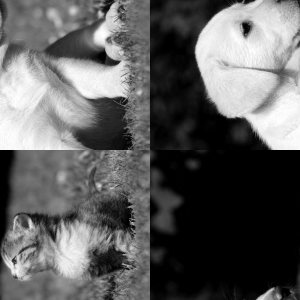
\includegraphics[height=150pt]{img.png}
\end{center}
\end{figure}

A grayscale image is just a matrix of numbers. Each `pixel' has
a certain \emph{intensity}. An intensity of 0 corresponds to black,
and an intensity of 255 corresponds to white. All numbers in between
correspond to increasingly lighter shades of gray. If you're curious,
color images work the same way, except we need three matrices, each
one representing the intensities of Red, Green and Blue.

Load the image on to Matlab:

\begin{minted}[bgcolor=bg]{octave}
    >> M = imread('img.png');
    >> size(M) % Gives the number of pixels in each direction 
               % (`dimensions')
    >> imshow(M) % Displays the image
\end{minted}

Of course, you don't need Matlab to check the image dimensions.

The objective of this exercise should be obvious: fix the image, given that
each `quarter' of the image is a 150 x 150 sub-image.

There is an important idea sitting behind this exercise: people in
fields like digital image processing or machine vision make careers
working with matrices. We hope this gives you a sense of why they are
so important.


\begin{minted}[bgcolor=bg]{octave}

% Read the image and obtain its dimensions:
M = imread('../figures/faceoff.png');
[R, C] = size(M);

% Break image into 'quarters'. We have done one
% for you.
%  ____ ____
% | q1 | q2 |
% |____|____|
% |    |    |
% |_q3_|_q4_|
%
%

% --------- YOUR CODE HERE --------- %
%q1 = 
%q2 = 
q3 = M(R/2+1:end, 1:R/2);
%q4 = 

% ---------------------------------- %

% Confirm that this command stacks the images
% appropriately
fixed_im = [q4, q3; q2, q1];

imwrite(fixed_im', 'fixedim.png');

\end{minted}

\end{document}